%!TeX root=../pridetop.tex
\chapter[Chapter \thechapter]{}
	
	
\begin{figure}[t!]
\centering
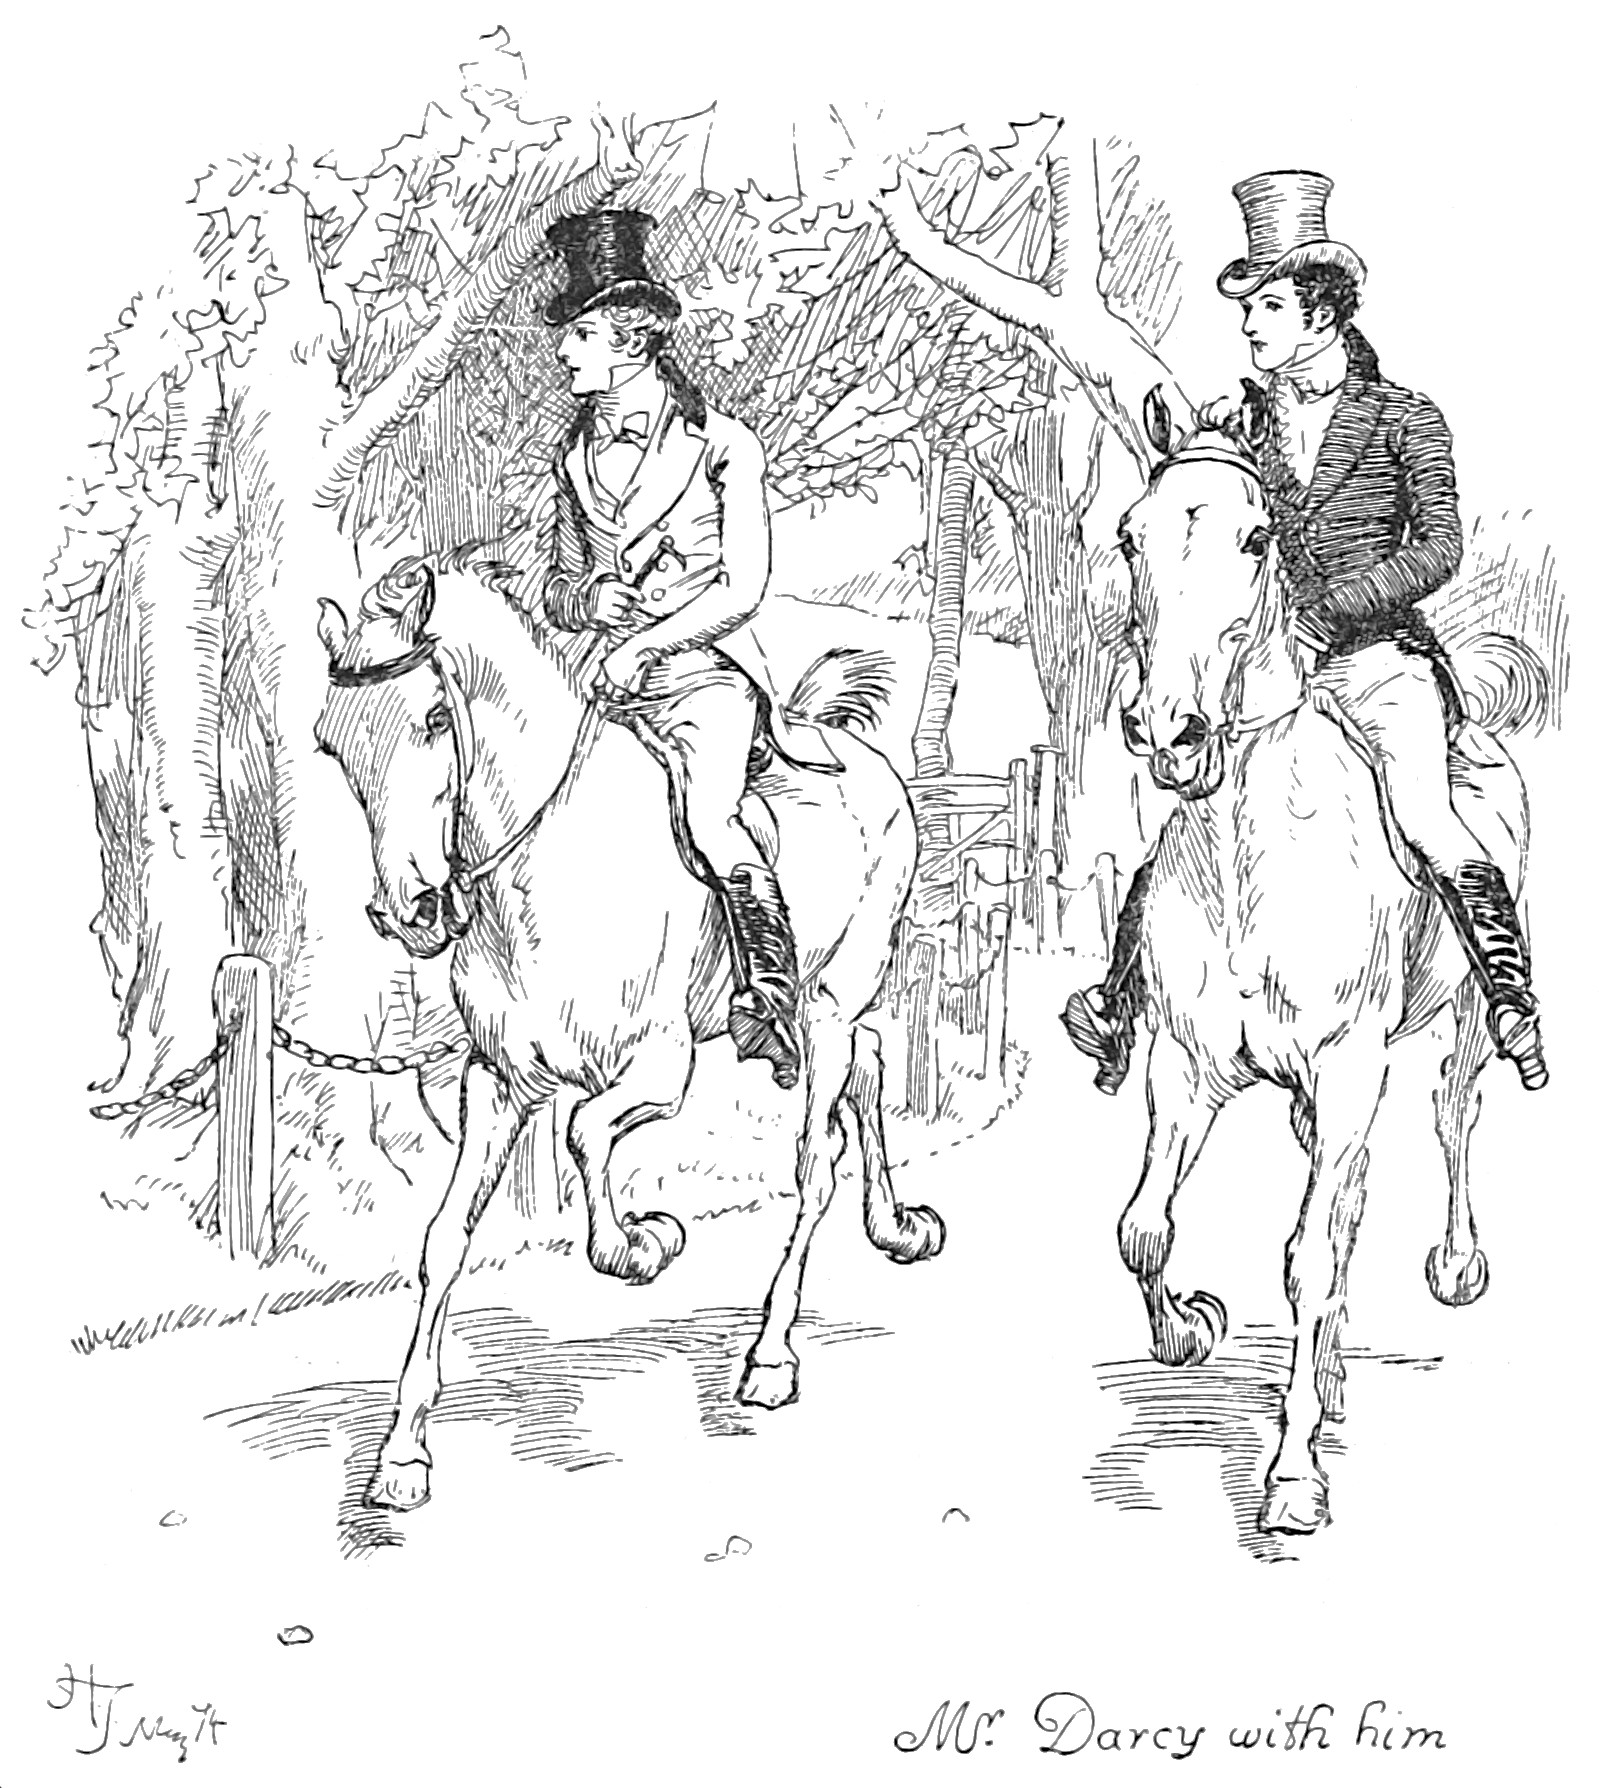
\includegraphics[width=.8\linewidth]{53top}
\captionlistentry{Mr Darcy with him}
\end{figure}


\lettrine[lines=6,image=true]{initials/chap53m}{r}  Wickham was so perfectly satisfied with this conversation, that he never again distressed himself, or provoked his dear sister Elizabeth, by introducing the subject of it; and she was pleased to find that she had said enough to keep him quiet.

\zz
The day of his and Lydia's departure soon came; and Mrs Bennet was forced to submit to a separation, which, as her husband by no means entered into her scheme of their all going to Newcastle, was likely to continue at least a twelvemonth.

»Oh, my dear Lydia,« she cried, »when shall we meet again?«

»Oh, Lord! I don't know. Not these two or three years, perhaps.«

»Write to me very often, my dear.«

»As often as I can. But you know married women have never much time for writing. My sisters may write to \textit{me}. They will have nothing else to do.«

Mr Wickham's adieus were much more affectionate than his wife's. He smiled, looked handsome, and said many pretty things.

»He is as fine a fellow,« said Mr Bennet, as soon as they were out of the house, »as ever I saw. He simpers, and smirks, and makes love to us all. I am prodigiously proud of him. I defy even Sir William Lucas himself to produce a more valuable son-in-law.«

The loss of her daughter made Mrs Bennet very dull for several days.

»I often think,« said she, »that there is nothing so bad as parting with one's friends. One seems so forlorn without them.«

»This is the consequence, you see, madam, of marrying a daughter,« said Elizabeth. »It must make you better satisfied that your other four are single.«

»It is no such thing. Lydia does not leave me because she is married; but only because her husband's regiment happens to be so far off. If that had been nearer, she would not have gone so soon.«

But the spiritless condition which this event threw her into was shortly relieved, and her mind opened again to the agitation of hope, by an article of news which then began to be in circulation. The housekeeper at Netherfield had received orders to prepare for the arrival of her master, who was coming down in a day or two, to shoot there for several weeks. Mrs Bennet was quite in the fidgets. She looked at Jane, and smiled, and shook her head, by turns.

»Well, well, and so Mr Bingley is coming down, sister,« (for Mrs Philips first brought her the news). »Well, so much the better. Not that I care about it, though. He is nothing to us, you know, and I am sure I never want to see him again. But, however, he is very welcome to come to Netherfield, if he likes it. And who knows what \textit{may} happen? But that is nothing to us. You know, sister, we agreed long ago never to mention a word about it. And so, it is quite certain he is coming?«

»You may depend on it,« replied the other, »for Mrs Nichols was in Meryton last night: I saw her passing by, and went out myself on purpose to know the truth of it; and she told me that it was certainly true. He comes down on Thursday, at the latest, very likely on Wednesday. She was going to the butcher's, she told me, on purpose to order in some meat on Wednesday, and she has got three couple of ducks just fit to be killed.«

Miss Bennet had not been able to hear of his coming without changing colour. It was many months since she had mentioned his name to Elizabeth; but now, as soon as they were alone together, she said,—

»I saw you look at me to-day, Lizzy, when my aunt told us of the present report; and I know I appeared distressed; but don't imagine it was from any silly cause. I was only confused for the moment, because I felt that I \textit{should} be looked at. I do assure you that the news does not affect me either with pleasure or pain. I am glad of one thing, that he comes alone; because we shall see the less of him. Not that I am afraid of \textit{myself}, but I dread other people's remarks.«

Elizabeth did not know what to make of it. Had she not seen him in Derbyshire, she might have supposed him capable of coming there with no other view than what was acknowledged; but she still thought him partial to Jane, and she wavered as to the greater probability of his coming there \textit{with} his friend's permission, or being bold enough to come without it.

»Yet it is hard,« she sometimes thought, »that this poor man cannot come to a house, which he has legally hired, without raising all this speculation! I \textit{will} leave him to himself.«

In spite of what her sister declared, and really believed to be her feelings, in the expectation of his arrival, Elizabeth could easily perceive that her spirits were affected by it. They were more disturbed, more unequal, than she had often seen them.

The subject which had been so warmly canvassed between their parents, about a twelvemonth ago, was now brought forward again.

»As soon as ever Mr Bingley comes, my dear,« said Mrs Bennet, »you will wait on him, of course.«

»No, no. You forced me into visiting him last year, and promised, if I went to see him, he should marry one of my daughters. But it ended in nothing, and I will not be sent on a fool's errand again.«

His wife represented to him how absolutely necessary such an attention would be from all the neighbouring gentlemen, on his returning to Netherfield.

»'Tis an \textit{etiquette} I despise,« said he. »If he wants our society, let him seek it. He knows where we live. I will not spend \textit{my} hours in running after my neighbours every time they go away and come back again.«

»Well, all I know is, that it will be abominably rude if you do not wait on him. But, however, that shan't prevent my asking him to dine here, I am determined. We must have Mrs Long and the Gouldings soon. That will make thirteen with ourselves, so there will be just room at table for him.«

Consoled by this resolution, she was the better able to bear her husband's incivility; though it was very mortifying to know that her neighbours might all see Mr Bingley, in consequence of it, before \textit{they} did. As the day of his arrival drew near,—

»I begin to be sorry that he comes at all,« said Jane to her sister. »It would be nothing; I could see him with perfect indifference; but I can hardly bear to hear it thus perpetually talked of. My mother means well; but she does not know, no one can know, how much I suffer from what she says. Happy shall I be when his stay at Netherfield is over!«

»I wish I could say anything to comfort you,« replied Elizabeth; »but it is wholly out of my power. You must feel it; and the usual satisfaction of preaching patience to a sufferer is denied me, because you have always so much.«

Mr Bingley arrived. Mrs Bennet, through the assistance of servants, contrived to have the earliest tidings of it, that the period of anxiety and fretfulness on her side be as long as it could. She counted the days that must intervene before their invitation could be sent—hopeless of seeing him before. But on the third morning after his arrival in Hertfordshire, she saw him from her dressing-room window enter the paddock, and ride towards the house.

Her daughters were eagerly called to partake of her joy. Jane resolutely kept her place at the table; but Elizabeth, to satisfy her mother, went to the window—she looked—she saw Mr Darcy with him, and sat down again by her sister.

»There is a gentleman with him, mamma,« said Kitty; »who can it be?«

»Some acquaintance or other, my dear, I suppose; I am sure I do not know.«

»La!« replied Kitty, »it looks just like that man that used to be with him before. Mr what's his name—that tall, proud man.«

»Good gracious! Mr Darcy!—and so it does, I vow. Well, any friend of Mr Bingley's will always be welcome here, to be sure; but else I must say that I hate the very sight of him.«

Jane looked at Elizabeth with surprise and concern. She knew but little of their meeting in Derbyshire, and therefore felt for the awkwardness which must attend her sister, in seeing him almost for the first time after receiving his explanatory letter. Both sisters were uncomfortable enough. Each felt for the other, and of course for themselves; and their mother talked on of her dislike of Mr Darcy, and her resolution to be civil to him only as Mr Bingley's friend, without being heard by either of them. But Elizabeth had sources of uneasiness which could not yet be suspected by Jane, to whom she had never yet had courage to show Mrs Gardiner's letter, or to relate her own change of sentiment towards him. To Jane, he could be only a man whose proposals she had refused, and whose merits she had undervalued; but to her own more extensive information, he was the person to whom the whole family were indebted for the first of benefits, and whom she regarded herself with an interest, if not quite so tender, at least as reasonable and just, as what Jane felt for Bingley. Her astonishment at his coming—at his coming to Netherfield, to Longbourn, and voluntarily seeking her again, was almost equal to what she had known on first witnessing his altered behaviour in Derbyshire.

The colour which had been driven from her face returned for half a minute with an additional glow, and a smile of delight added lustre to her eyes, as she thought for that space of time that his affection and wishes must still be unshaken; but she would not be secure.

»Let me first see how he behaves,« said she; »it will then be early enough for expectation.«

She sat intently at work, striving to be composed, and without daring to lift up her eyes, till anxious curiosity carried them to the face of her sister as the servant was approaching the door. Jane looked a little paler than usual, but more sedate than Elizabeth had expected. On the gentlemen's appearing, her colour increased; yet she received them with tolerable ease, and with a propriety of behaviour equally free from any symptom of resentment, or any unnecessary complaisance.

Elizabeth said as little to either as civility would allow, and sat down again to her work, with an eagerness which it did not often command. She had ventured only one glance at Darcy. He looked serious as usual; and, she thought, more as he had been used to look in Hertfordshire, than as she had seen him at Pemberley. But, perhaps, he could not in her mother's presence be what he was before her uncle and aunt. It was a painful, but not an improbable, conjecture.

Bingley she had likewise seen for an instant, and in that short period saw him looking both pleased and embarrassed. He was received by Mrs Bennet with a degree of civility which made her two daughters ashamed, especially when contrasted with the cold and ceremonious politeness of her courtesy and address of his friend.

Elizabeth particularly, who knew that her mother owed to the latter the preservation of her favourite daughter from irremediable infamy, was hurt and distressed to a most painful degree by a distinction so ill applied.

Darcy, after inquiring of her how Mr and Mrs Gardiner did—a question which she could not answer without confusion—said scarcely anything. He was not seated by her: perhaps that was the reason of his silence; but it had not been so in Derbyshire. There he had talked to her friends when he could not to herself. But now several minutes elapsed, without bringing the sound of his voice; and when occasionally, unable to resist the impulse of curiosity, she raised her eyes to his face, she as often found him looking at Jane as at herself, and frequently on no object but the ground. More thoughtfulness and less anxiety to please, than when they last met, were plainly expressed. She was disappointed, and angry with herself for being so.

»Could I expect it to be otherwise?« said she. »Yet why did he come?«

She was in no humour for conversation with anyone but himself; and to him she had hardly courage to speak.

She inquired after his sister, but could do no more.

»It is a long time, Mr Bingley, since you went away,« said Mrs Bennet.

He readily agreed to it.

»I began to be afraid you would never come back again. People \textit{did} say, you meant to quit the place entirely at Michaelmas; but, however, I hope it is not true. A great many changes have happened in the neighbourhood since you went away. Miss Lucas is married and settled: and one of my own daughters. I suppose you have heard of it; indeed, you must have seen it in the papers. It was in the \textit{Times} and the \textit{Courier}, I know; though it was not put in as it ought to be. It was only said, »Lately, George Wickham, Esq., to Miss Lydia Bennet,« without there being a syllable said of her father, or the place where she lived, or anything. It was my brother Gardiner's drawing up, too, and I wonder how he came to make such an awkward business of it. Did you see it?«

Bingley replied that he did, and made his congratulations. Elizabeth dared not lift up her eyes. How Mr Darcy looked, therefore, she could not tell.

»It is a delightful thing, to be sure, to have a daughter well married,« continued her mother; »but at the same time, Mr Bingley, it is very hard to have her taken away from me. They are gone down to Newcastle, a place quite northward it seems, and there they are to stay, I do not know how long. His regiment is there; for I suppose you have heard of his leaving the ——shire, and of his being gone into the Regulars. Thank heaven! he has \textit{some} friends, though, perhaps, not so many as he deserves.«

Elizabeth, who knew this to be levelled at Mr Darcy, was in such misery of shame that she could hardly keep her seat. It drew from her, however, the exertion of speaking, which nothing else had so effectually done before; and she asked Bingley whether he meant to make any stay in the country at present. A few weeks, he believed.

»When you have killed all your own birds, Mr Bingley,« said her mother, »I beg you will come here and shoot as many as you please on Mr Bennet's manor. I am sure he will be vastly happy to oblige you, and will save all the best of the coveys for you.«

Elizabeth's misery increased at such unnecessary, such officious attention! Were the same fair prospect to arise at present, as had flattered them a year ago, everything, she was persuaded, would be hastening to the same vexatious conclusion. At that instant she felt, that years of happiness could not make Jane or herself amends for moments of such painful confusion.

»The first wish of my heart,« said she to herself, »is never more to be in company with either of them. Their society can afford no pleasure that will atone for such wretchedness as this! Let me never see either one or the other again!«

Yet the misery, for which years of happiness were to offer no compensation, received soon afterwards material relief, from observing how much the beauty of her sister rekindled the admiration of her former lover. When first he came in, he had spoken to her but little, but every five minutes seemed to be giving her more of his attention. He found her as handsome as she had been last year; as good-natured, and as unaffected, though not quite so chatty. Jane was anxious that no difference should be perceived in her at all, and was really persuaded that she talked as much as ever; but her mind was so busily engaged, that she did not always know when she was silent.

When the gentlemen rose to go away, Mrs Bennet was mindful of her intended civility, and they were invited and engaged to dine at Longbourn in a few days' time.

»You are quite a visit in my debt, Mr Bingley,« she added; »for when you went to town last winter, you promised to take a family dinner with us as soon as you returned. I have not forgot, you see; and I assure you I was very much disappointed that you did not come back and keep your engagement.«

Bingley looked a little silly at this reflection, and said something of his concern at having been prevented by business. They then went away.

Mrs Bennet had been strongly inclined to ask them to stay and dine there that day; but, though she always kept a very good table, she did not think anything less than two courses could be good enough for a man on whom she had such anxious designs, or satisfy the appetite and pride of one who had ten thousand a year.